%%%%%%%%%%%%%%%%%%%%%%%%%%%%%%%%%%%%%%%%%%%%%%%%%%%%%%%%%%%%%%%%%%%%%%
% ReinforcePeace: ARC-AGI-3 report, COMS4061A/COMS7071A 2026
% Built on the official RLJ/RLC 2026 template (rlj.sty / rlj.bst, Version 2026.1).
% Brief requirements honoured here:
%   - cover page disabled (\makeCover commented out below)
%   - authors shown with student emails, so the [preprint] option is used
%     (de-anonymised, no RLJ/RLC branding claims)
%   - max 8 pages of main text before the references; template fonts/margins untouched
% Red [TODO: ...] markers flag everything that still needs results or confirmation.
%%%%%%%%%%%%%%%%%%%%%%%%%%%%%%%%%%%%%%%%%%%%%%%%%%%%%%%%%%%%%%%%%%%%%%

\documentclass[10pt]{article}

\usepackage[preprint]{rlj}   % de-anonymised: the brief requires the author list

\usepackage{amssymb}
\usepackage{mathtools}
\usepackage{graphicx}
\usepackage{subcaption}
\usepackage[space]{grffile}
\usepackage{url}
\usepackage{xurl}        % lets long URLs (the Paper Track link) break across lines
\usepackage{booktabs}

% Visible marker for unfinished content. Search for "TODO" before submitting.
\newcommand{\todo}[1]{\textcolor{red}{[TODO: #1]}}

%%%%%%%%%%%%%%%%%%%%%%%%%%%%%%%%%%%%%%%%%%%%%%%%%%%%%%%%%%%%%%%%
% Meta-data
%%%%%%%%%%%%%%%%%%%%%%%%%%%%%%%%%%%%%%%%%%%%%%%%%%%%%%%%%%%%%%%%

\title{Memory and Count-Based Exploration for Sparse-Reward Interactive Reasoning: DQN versus Maskable PPO on ARC-AGI-3}

\setrunningtitle{Memory and Exploration for ARC-AGI-3}

\author{Banele Mkhize\textsuperscript{1}, Elias Sepuru\textsuperscript{1}, Paballo\textsuperscript{1}}

\coverPageAuthor{Banele Mkhize, Elias Sepuru, Paballo}

% Student emails use student numbers, as the brief requires. TODO: confirm the email format.
\emails{\{2663814, 1427726, 3134698\}@students.wits.ac.za}

\affiliations{
$^{1}$\textbf{School of Computer Science and Applied Mathematics, University of the Witwatersrand, South Africa}
\par
Kaggle team: \textbf{ReinforcePeace}
}

% The cover page is disabled for this assignment, so the contribution boxes, keywords and summary
% below are not printed. They are kept filled in so the file stays valid for the template.
\contribution{
    An empirical comparison of a course algorithm (DQN) and a non-course algorithm (Maskable PPO) on ARC-AGI-3, each improved in two evidence-motivated stages (frame-stacking memory, then a count-based novelty bonus) with a novelty-only ablation
    }
    {
    Both algorithms, the memory wrapper and the count-based bonus are established methods; the contribution is their controlled evaluation on held-out ARC-AGI-3 games
    }

\keywords{ARC-AGI-3, sparse reward, exploration, partial observability, DQN, PPO, action masking}

\summary{See abstract.}

%%%%%%%%%%%%%%%%%%%%%%%%%%%%%%%%%%%%%%%%%%%%%%%%%%%%%%%%%%%%%%%%
\begin{document}

% \makeCover  % Disabled: the assignment brief requires no cover page.
\maketitle

\begin{abstract}
ARC-AGI-3 drops an agent into unfamiliar grid games with no instructions, no stated goal and no reward other than a counter of completed levels. We study how far standard deep reinforcement learning gets in this setting, and which changes help. We compare Deep Q-Networks (DQN), an algorithm from the course, with Proximal Policy Optimisation using invalid-action masking (Maskable PPO), an algorithm outside the course. Each starts from a baseline and is improved twice, with each change motivated by the previous stage's evidence: first memory, by stacking recent screens, then a count-based novelty bonus to address the sparse reward. A novelty-only ablation isolates the bonus. All agents are trained on 19 public games for 50,000 steps per seed and evaluated on 6 held-out games over 3 seeds, against a random policy. No agent, including the random reference, completed a level on a held-out game, so neither improvement produced a measurable gain at this budget. The experiments still separate the algorithms: during training, Maskable PPO completed about twice as many levels as DQN, and on held-out games DQN with memory or novelty repeatedly collapsed onto an action the game does not offer, spending up to all 500 steps on it, while masked PPO never wasted an action. We report these negative results, their likely causes, and the logging and budget limitations that bound our conclusions. Code: submitted with this report (Kaggle notebook of submission 57654331).
\end{abstract}

%%%%%%%%%%%%%%%%%%%%%%%%%%%%%%%%%%%%%%%%%%%%%%%%%%%%%%%%%%%%%%%%
\section{Introduction}
\label{sec:introduction}
%%%%%%%%%%%%%%%%%%%%%%%%%%%%%%%%%%%%%%%%%%%%%%%%%%%%%%%%%%%%%%%%

ARC-AGI-3 \citep{arcprize2026} measures how efficiently an agent learns an unfamiliar interactive task, following the view that intelligence is skill-acquisition efficiency rather than skill itself \citep{chollet2019measure}. Each game is a grid of up to $64\times 64$ cells in 16 colours. The agent is told nothing about what its actions do or what counts as success; the only feedback is a counter that increases when a level is completed. The official score rewards efficiency: a completed level scores the squared ratio of the actions a human needed to the actions the agent needed.

Two properties make this hard for reinforcement learning (RL). First, reward is extremely sparse: until the first level is completed by chance, every reward is zero and value-based and policy-gradient methods receive no learning signal. Second, the screen does not always show the full state (for example, which switches have been pressed), so the problem is partially observable.

\textbf{Research question.} Starting from two standard deep RL baselines, do memory and count-based exploration improve level completion on held-out ARC-AGI-3 games, and does their effect differ between a value-based method without action masking (DQN) and a policy-gradient method with masking (Maskable PPO)?

\textbf{Contributions.} (i) A Gymnasium adapter for ARC-AGI-3 that fixes the observation, action abstraction, availability mask, reward and termination semantics (Section~\ref{sec:formulation}). (ii) Two baselines and two improvement stages per algorithm, plus a novelty-only ablation, evaluated on held-out games over three seeds against a random policy (Sections~\ref{sec:methods}--\ref{sec:results}). (iii) A negative result with diagnosis: at a 50,000-step budget no variant completes a held-out level; masking separates the algorithms clearly, while memory and novelty show no measurable benefit and make unmasked DQN more prone to collapsing onto unavailable actions (Section~\ref{sec:results}).

%%%%%%%%%%%%%%%%%%%%%%%%%%%%%%%%%%%%%%%%%%%%%%%%%%%%%%%%%%%%%%%%
\section{Background}
\label{sec:background}
%%%%%%%%%%%%%%%%%%%%%%%%%%%%%%%%%%%%%%%%%%%%%%%%%%%%%%%%%%%%%%%%

\textbf{DQN} \citep{mnih2015human} learns an action-value function $Q_\theta(s,a)$ with a convolutional network. Transitions are stored in a replay buffer, and the network is regressed towards the target $r + \gamma \max_{a'} Q_{\bar\theta}(s',a')$, where $\bar\theta$ is a periodically refreshed copy of the weights. It acts $\epsilon$-greedily during training and greedily during evaluation. DQN scores every action and has no built-in way to exclude actions the game does not currently offer.

\textbf{PPO} \citep{schulman2017proximal} learns a stochastic policy $\pi_\theta(a\mid s)$ and a value function $V_\phi(s)$. It alternates between collecting a batch of on-policy experience and several epochs of minibatch updates of the clipped surrogate objective
\begin{equation}
L^{\text{CLIP}}(\theta) = \mathbb{E}_t\!\left[\min\!\big(\rho_t(\theta)\hat A_t,\ \operatorname{clip}(\rho_t(\theta), 1-\varepsilon, 1+\varepsilon)\hat A_t\big)\right],
\qquad \rho_t(\theta)=\frac{\pi_\theta(a_t\mid s_t)}{\pi_{\theta_\text{old}}(a_t\mid s_t)},
\end{equation}
where $\hat A_t$ is a generalised advantage estimate. Clipping the probability ratio stops any single update from moving the policy far from the one that collected the data. An entropy bonus keeps the policy stochastic. \textbf{Invalid-action masking} \citep{huang2022closer} sets the logits of unavailable actions to $-\infty$ before the softmax, so they receive zero probability both when acting and in the gradient.

\textbf{Count-based exploration} pays an intrinsic bonus that shrinks with how often a state has been visited, of the form $\beta/\sqrt{N(s)}$ \citep{strehl2008analysis, bellemare2016unifying}. For high-dimensional observations, counts can be kept over hashed observations \citep{tang2017exploration}.

\textbf{Memory.} When the observation does not determine the state, a policy conditioned on the current observation alone has a performance ceiling. Stacking the last $k$ observations is the standard remedy \citep{mnih2015human}; recurrent networks are an alternative \citep{hausknecht2015deep}. Frame stacking's window must grow with how far back the relevant information lies; Adaptive Stacking \citep{nanguetasse2025beyond} instead keeps a small stack and learns which memories to remove, so it can keep informative old observations.

%%%%%%%%%%%%%%%%%%%%%%%%%%%%%%%%%%%%%%%%%%%%%%%%%%%%%%%%%%%%%%%%
\section{Problem formulation}
\label{sec:formulation}
%%%%%%%%%%%%%%%%%%%%%%%%%%%%%%%%%%%%%%%%%%%%%%%%%%%%%%%%%%%%%%%%

The official ARC-AGI-3 interface is not a Gymnasium environment, so we wrote an adapter, \texttt{ArcGymEnv} \citep{towers2024gymnasium}, which defines the decision process our agents solve. Each reset samples one game uniformly from the given list.

\textbf{Observation.} The last grid of the returned frame (a frame can contain several grids of an animation), zero-padded to $64\times64$ and multiplied by 16 so the 16 colour indices spread over $0$--$240$: a $1\times64\times64$ \texttt{uint8} image. If a frame arrives with no grid, the previous observation is repeated.

\textbf{Actions.} 70 discrete actions: the five simple actions \texttt{ACTION1}--\texttt{ACTION5}, the undo action \texttt{ACTION7}, and 64 clicks (\texttt{ACTION6}) at the centres of an $8\times8$ grid of $8\times8$-cell blocks, $(x, y) = (8c+4,\ 8r+4)$. A free click has 4,096 targets; the coarse grid makes exploration tractable at the cost of making precise off-centre clicks impossible.

\textbf{Action availability.} Each frame lists the actions the game currently offers. The adapter exposes this as a 70-entry mask. An action outside the mask is not sent to the game: the observation is unchanged, the reward is 0, and the step counts against the step budget. Maskable PPO never selects such actions; DQN can.

\textbf{Reward.} The change in the levels-completed counter, $r_t = L_{t+1} - L_t$. Nothing else is added in the baselines. The novelty bonus (Section~\ref{sec:methods}) is used during training only and is never reported as performance.

\textbf{Termination.} An episode \emph{terminates} when the game reports \texttt{WIN} or \texttt{GAME\_OVER}, and is \emph{truncated} after 500 steps. The two are kept separate so that bootstrapped value targets are not cut off at our own step cap.

\textbf{Partial observability.} The screen need not reveal the full game state, so the process is a POMDP; the memory improvement targets this.

\textbf{What persists.} Network weights are learned offline on the training games and frozen for evaluation; there is no online learning or adaptation at test time. Frame-stacking memory persists within an episode and is reset with it. Novelty counts accumulate over a whole training run and do not exist at evaluation. Nothing persists between games or between evaluation runs.

%%%%%%%%%%%%%%%%%%%%%%%%%%%%%%%%%%%%%%%%%%%%%%%%%%%%%%%%%%%%%%%%
\section{Methods}
\label{sec:methods}
%%%%%%%%%%%%%%%%%%%%%%%%%%%%%%%%%%%%%%%%%%%%%%%%%%%%%%%%%%%%%%%%

Both learners use the Stable-Baselines3 implementations \citep{raffin2021stable}: \texttt{DQN} and \texttt{MaskablePPO} from sb3-contrib, each with the default Nature-CNN feature extractor (\texttt{CnnPolicy}). We wrote the adapter, wrappers, evaluation protocol, experiment runner and Kaggle agent ourselves (Appendix~\ref{sec:supp-reuse}).

\textbf{Reference policy.} \texttt{random\_v0} picks uniformly among the currently available actions. It is a sanity check, not a baseline learner.

\textbf{Baselines (v0).} DQN and Maskable PPO on the adapter as described, with the hyperparameters in Table~\ref{tab:hyperparameters}.
For DQN, what is learned is $Q_\theta$; learning happens every 4 environment steps from replayed transitions once 1,000 steps have been collected; decisions are greedy in $Q_\theta$ (with $\epsilon$-random actions while training). For PPO, what is learned is the policy and value networks; learning happens after every 512 collected steps, in 10 epochs of minibatches of 64; decisions sample from the masked policy during training and take its most probable legal action at evaluation.

\textbf{How the improvements were chosen.} Both improvements were fixed before the baselines were trained, on two a~priori arguments: hidden state makes single screens ambiguous (memory), and zero reward before the first success gives no learning signal (exploration). Time did not allow a fully sequential design in which v0 results choose the v1 change. We therefore state, for each change, the limitation it targets and the baseline evidence consistent with it.

\textbf{Improvement 1: memory (v1).} \emph{Limitation:} a policy that sees one screen cannot act on information that is no longer displayed. In the baselines, deterministic agents produced identical action counts on most held-out games regardless of algorithm (Section~\ref{sec:results}), consistent with policies that do not react to game progress. \emph{Hypothesis:} conditioning on recent screens lets the agent distinguish situations that look identical on the current screen. \emph{Intervention:} the observation becomes the last $k=4$ screens, $4\times64\times64$, oldest dropped first, refilled with the first screen on reset.

\textbf{Improvement 2: count-based novelty (v2).} \emph{Limitation:} the baselines completed only 3 to 17 levels in 50,000 training steps, so reward is almost always zero. \emph{Hypothesis:} a bonus for rarely seen screens makes exploration systematic, so levels are completed more often and learning can begin. \emph{Intervention:} each single screen (before stacking) is hashed (MD5 of its bytes) and counted over the whole training run; the training reward becomes $r_t + \beta / \sqrt{N(o_{t+1})}$ with $\beta = 0.1$. The bonus wraps the adapter inside the frame stack, so counts are over single screens, not over 4-screen sequences.

\textbf{Ablation.} \texttt{v2\_novelty\_only} applies the novelty bonus without memory. Comparing v0, v1, v2 and the ablation separates the contribution of each change, and is run separately for each algorithm.

We also implemented Adaptive Stacking as an alternative memory (for DQN the joint choice of action and slot is flattened to $70\times4=280$ actions), but did not run it within the time budget.

\textbf{Kaggle agent.} The submitted agent is the \texttt{ppo\_v1\_memory} model of seed 2, chosen because it completed the most levels during training (19); no held-out result was used to choose it. It reproduces the adapter's preprocessing, mask and click mapping exactly, keeps the last four screens, presses \texttt{RESET} at the start and after game over, and stops on a win. Unlike our local evaluation it samples from the masked policy instead of taking the most probable action: on Kaggle a game is retried after game over, and a deterministic policy would replay the same failed attempt on every retry.

\begin{table}[t]
\caption{Hyperparameters. Unlisted values are Stable-Baselines3 2.9.0 defaults.}
\label{tab:hyperparameters}
\begin{center}
\small
\begin{tabular}{lll}
\toprule
 & \textbf{DQN} & \textbf{Maskable PPO} \\
\midrule
Policy network & Nature CNN (\texttt{CnnPolicy}) & Nature CNN (\texttt{CnnPolicy}) \\
Learning rate & $10^{-4}$ & $3\times10^{-4}$ \\
Discount $\gamma$ & 0.99 & 0.99 \\
Batch size & 32 & 64 \\
Replay buffer / rollout & 20,000 transitions & 512 steps \\
Learning starts / epochs & 1,000 steps & 10 epochs per rollout \\
Train frequency & every 4 steps & every 512 steps \\
Target network update & every 1,000 steps & n/a \\
Exploration & $\epsilon$: $1.0 \to 0.05$ over 30\% of training & entropy coefficient 0.01 \\
Clip range / GAE $\lambda$ & n/a & 0.2 / 0.95 \\
\midrule
Training budget & \multicolumn{2}{l}{50,000 environment steps per seed; 3 seeds (0, 1, 2)} \\
Episode cap & \multicolumn{2}{l}{500 steps (truncation)} \\
Memory ($v1$, $v2$) & \multicolumn{2}{l}{last $k=4$ screens} \\
Novelty bonus ($v2$) & \multicolumn{2}{l}{$\beta=0.1$, MD5 hash of single screens, counts kept for the whole run} \\
\bottomrule
\end{tabular}
\end{center}
\end{table}

%%%%%%%%%%%%%%%%%%%%%%%%%%%%%%%%%%%%%%%%%%%%%%%%%%%%%%%%%%%%%%%%
\section{Experimental setup}
\label{sec:setup}
%%%%%%%%%%%%%%%%%%%%%%%%%%%%%%%%%%%%%%%%%%%%%%%%%%%%%%%%%%%%%%%%

\textbf{Games.} The 25 public games are sorted by identifier and every fourth game is held out: the 6 held-out games (\texttt{cn04}, \texttt{ka59}, \texttt{m0r0}, \texttt{sb26}, \texttt{su15}, \texttt{vc33}) are never used for training; the other 19 are. The full identifiers, including versions, are listed in Appendix~\ref{sec:supp-games}.

\textbf{Protocol.} Fixed before any improvement was evaluated. Each trained model plays every held-out game once (1 episode per game) with the same 500-step cap, acting deterministically. Every run is recorded, including those that complete nothing. Each evaluation seeds all random number generators with the run's seed, so results are repeatable. We record levels completed (out of the game's total), whether the game was won, actions used, invalid actions, and wall time.

\textbf{Scoring.} Our primary local metric is levels completed on held-out games, with actions used and invalid actions as secondary measures. The official ARC-AGI-3 score is computed per level from human and agent action counts on the hidden evaluation games; we report it only as returned by Kaggle, separately from local numbers. Training curves come from per-episode logs of reward and episode length; for the novelty versions the logged reward includes the bonus, so it is not a level count.

\textbf{Compute.} All training and evaluation ran locally on one laptop CPU (Intel Core, 6 cores / 12 threads, no GPU), Python 3.13.5, PyTorch 2.9.1 (CPU), Stable-Baselines3 and sb3-contrib 2.9.0, Gymnasium 1.4.0, \texttt{arc-agi} 0.9.9 and \texttt{arcengine} 0.9.3, with games run offline from local copies. Training took 174 minutes for all 24 runs (6.0 to 10.2 minutes per run, mean 7.3); held-out evaluation took 71 seconds for all 24 runs plus 1.5 seconds for the random policy.

\textbf{Fair comparison.} All versions use the same games, training budget, episode cap, seeds and evaluation protocol. The final checkpoint of each run is evaluated; no checkpoint selection is done on held-out games.

%%%%%%%%%%%%%%%%%%%%%%%%%%%%%%%%%%%%%%%%%%%%%%%%%%%%%%%%%%%%%%%%
\section{Results}
\label{sec:results}
%%%%%%%%%%%%%%%%%%%%%%%%%%%%%%%%%%%%%%%%%%%%%%%%%%%%%%%%%%%%%%%%

\textbf{Reference policy.} The random policy completed no level on any held-out game in any seed. On four of the six games the episode ended after exactly the same number of actions in every seed (\texttt{cn04}: 75, \texttt{ka59}: 100, \texttt{m0r0}: 151, \texttt{vc33}: 50), which indicates a fixed per-attempt action budget independent of the actions taken; \texttt{su15} ended after 39--40 actions and \texttt{sb26} always ran to the 500-step cap. Running out of actions ends an attempt with zero reward, which to the agent is indistinguishable from an attempt in which nothing has happened yet.

\textbf{Held-out games: no level completed by any agent.} Across all 8 learned versions, 3 seeds and 6 held-out games, and for the random policy, no level was completed and no game was won (Table~\ref{tab:results}). The official local score is therefore zero for every version, and the improvements cannot be ranked on completion. The remaining measures still differ.

\begin{table}[t]
\caption{Held-out and training results. Held-out columns: mean $\pm$ standard deviation across the 3 seeds of each seed's mean over the 6 held-out games. Training levels: levels completed during the 50,000 training steps, per seed; for novelty versions the logged reward includes the bonus, so levels were not recoverable (n/a).}
\label{tab:results}
\begin{center}
\small
\begin{tabular}{llcccc}
\toprule
 & & \multicolumn{3}{c}{\textbf{Held-out (6 games)}} & \textbf{Training} \\
\textbf{Alg.} & \textbf{Version} & \textbf{Levels} & \textbf{Actions used} & \textbf{Invalid actions} & \textbf{Levels, seeds 0/1/2} \\
\midrule
Random & reference & 0 & $152.6 \pm 0.1$ & 0 & n/a \\
\midrule
DQN & v0 baseline & 0 & $153.1 \pm 3.1$ & $0.0 \pm 0.0$ & 3 / 7 / 10 \\
 & v1 memory & 0 & $202.3 \pm 88.3$ & $27.8 \pm 48.1$ & 5 / 0 / 1 \\
 & v2 memory + novelty & 0 & $202.3 \pm 88.3$ & $83.3 \pm 144.3$ & n/a \\
 & novelty only & 0 & $279.3 \pm 43.3$ & $166.7 \pm 144.3$ & n/a \\
\midrule
PPO & v0 baseline & 0 & $151.3 \pm 0.0$ & 0 & 6 / 15 / 17 \\
 & v1 memory & 0 & $151.3 \pm 0.0$ & 0 & 11 / 8 / 19 \\
 & v2 memory + novelty & 0 & $127.1 \pm 42.0$ & 0 & n/a \\
 & novelty only & 0 & $151.3 \pm 0.0$ & 0 & n/a \\
\bottomrule
\end{tabular}
\end{center}
\end{table}

\textbf{Reference policy and game structure.} On four of the six held-out games every agent, learned or random, used exactly the same number of actions in every seed (\texttt{cn04}: 75, \texttt{ka59}: 100, \texttt{m0r0}: 151, \texttt{vc33}: 50 when no invalid actions occur). These games end each attempt after a fixed action budget, whatever is pressed. Running out ends the episode with zero reward, which to the agent is indistinguishable from an episode in which nothing has happened yet. \texttt{su15} ends sooner under PPO (32 actions) than under random play (39), and \texttt{sb26} usually runs to our 500-step cap.

\textbf{Baselines.} During training both baselines completed levels only rarely (Figure~\ref{fig:training}): DQN 3, 7 and 10 levels per seed, PPO 6, 15 and 17, in about 150 (DQN) and 255 (PPO) training episodes. PPO completed about twice as many levels and its episodes were shorter (mean 196 versus 326 steps). On held-out games both baselines behaved like the random policy: identical action counts and no invalid actions.

\begin{figure}[t]
    \centering
    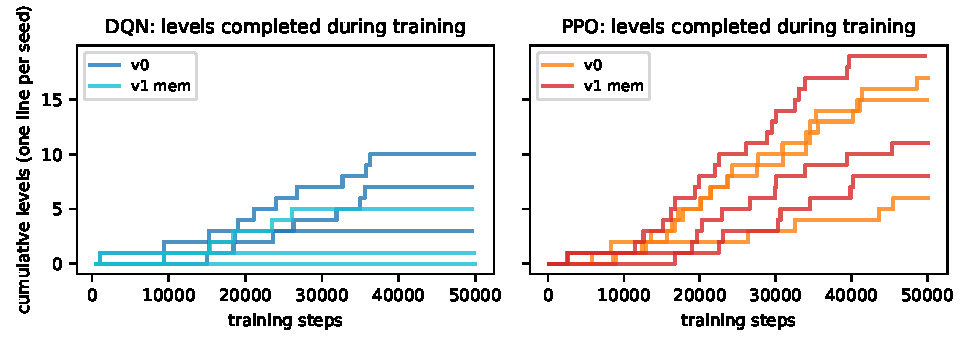
\includegraphics[width=\linewidth]{figures/training_levels.pdf}
    \caption{Cumulative levels completed during training (true game reward), one line per seed, for the versions without the novelty bonus. Levels are rare for every run; PPO completes more than DQN; memory makes no consistent difference for PPO and reduces completions for DQN, with large seed-to-seed variation.}
    \label{fig:training}
\end{figure}

\textbf{Improvement 1, memory.} For PPO, memory left training completions unchanged on average (11, 8, 19 versus 6, 15, 17 levels; means 12.7 for both) and left held-out behaviour identical to the baseline. For DQN, completions fell (5, 0, 1 versus 3, 7, 10), within a large seed spread, and one seed collapsed on \texttt{vc33} onto an action the game does not offer, pressing it until the 500-step cap. The hypothesis that memory helps is not supported at this budget: the observable failures were not caused by missing history.

\textbf{Improvement 2, novelty.} The bonus dominated the training reward: each novelty episode returned about 10 in bonus, against at most a few completed levels in an entire baseline run. We did not log the true reward separately per episode, so we cannot say whether novelty changed how often levels were completed during training (Section~\ref{sec:discussion}). Its behavioural effect is visible: training episodes became shorter for DQN (mean about 250 versus 326 steps; Figure~\ref{fig:length}), which is consistent with the agent pressing buttons that change the screen, and so use up the game's action budget, more often. On held-out games novelty did not complete any level.

\begin{figure}[t]
    \centering
    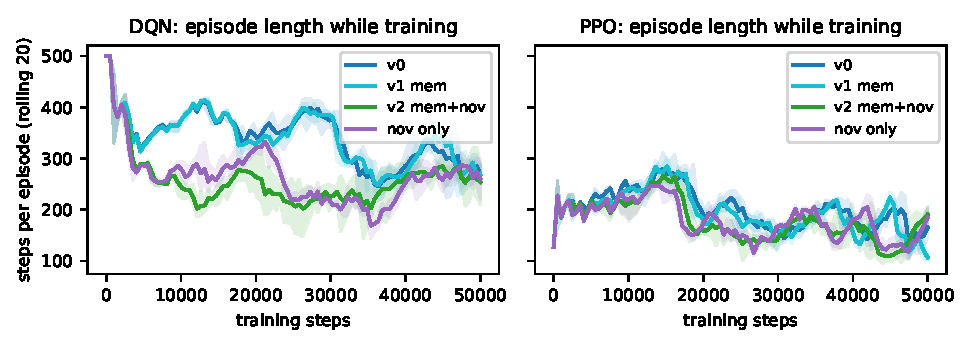
\includegraphics[width=\linewidth]{figures/episode_length.pdf}
    \caption{Training episode length (rolling mean of 20 episodes; line: mean over seeds; band: min to max). The novelty bonus (green, purple) shortens DQN's episodes early in training; for PPO all versions are similar.}
    \label{fig:length}
\end{figure}

\textbf{Ablation and failure case: DQN collapses onto unavailable actions.} Figure~\ref{fig:invalid} isolates the clearest effect in the study. Masked PPO never pressed an unavailable action in any version. DQN v0 did not either, but every DQN change increased the number of seed--game pairs in which the greedy policy locked onto an action the game does not offer and pressed it for all remaining steps: one with memory (\texttt{vc33}), three with memory and novelty, and six with novelty alone (\texttt{sb26}, \texttt{su15} and \texttt{vc33} in two seeds each). Because such presses never reach the game, the game's own action budget is never spent, and the episode only ends at our cap, which is why these versions use more actions in Table~\ref{tab:results}. The ablation therefore attributes the increase mainly to the novelty bonus rather than to memory. We did not establish why novelty makes this collapse more frequent; one candidate is that the bonus inflates action values in training games that offer different actions, so an action whose value was learned elsewhere wins the greedy choice on a game that does not offer it.

\begin{figure}[t]
    \centering
    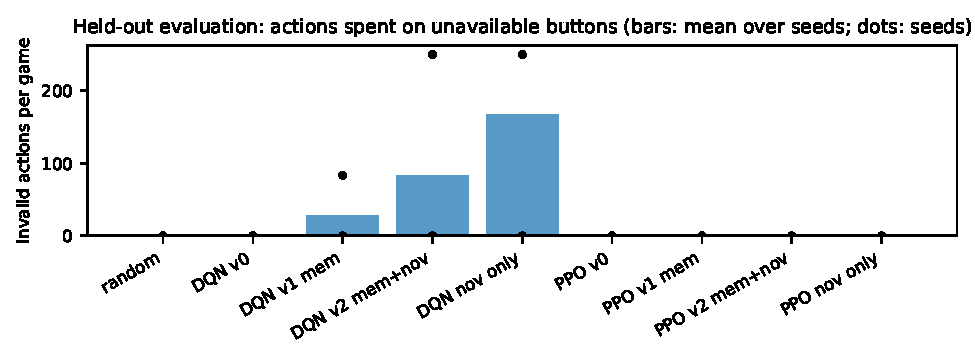
\includegraphics[width=\linewidth]{figures/invalid_actions.pdf}
    \caption{Held-out evaluation: mean invalid actions per game for each version (bars), with each seed as a dot. Only unmasked DQN with memory and/or novelty presses unavailable actions; a seed at 250 spent its whole 500-step budget on one unavailable action in three of the six games.}
    \label{fig:invalid}
\end{figure}

\textbf{Kaggle.} On the hidden evaluation games, the starter kit's random agent (submission 57627136) scored 0.07 on the public leaderboard, and our trained Maskable PPO agent (submission 57654331, the nominated entry) scored 0.00, consistent with its zero held-out completions locally. The random agent retries with clicks anywhere on the $64\times64$ grid, while our agent can only click 64 block centres and samples from a policy that learned little, so on these hidden games it explored less widely than random. These are official Kaggle scores and are not comparable with our local held-out numbers. Identifiers and timestamps are in Appendix~\ref{sec:supp-evidence}.

%%%%%%%%%%%%%%%%%%%%%%%%%%%%%%%%%%%%%%%%%%%%%%%%%%%%%%%%%%%%%%%%
\section{Discussion and limitations}
\label{sec:discussion}
%%%%%%%%%%%%%%%%%%%%%%%%%%%%%%%%%%%%%%%%%%%%%%%%%%%%%%%%%%%%%%%%

\textbf{Comparing the final agents.} Neither final agent generalised to held-out games at this budget, so the comparison rests on secondary evidence. PPO's strengths here come from masking and on-policy sampling: it never wastes an action, completed about twice as many training levels, and finished more training episodes in the same budget. DQN's weakness is the reverse: without a mask, a greedy policy can lock onto an unavailable action and stall an entire episode, and every change we made increased this risk. In interaction efficiency neither agent can be scored, since neither completed a held-out level; in compute both cost about 7 minutes per 50,000-step run on a CPU, and evaluation is negligible.

\textbf{Why the improvements did not help.} The most likely explanation is budget. With 3 to 19 completed levels spread over 19 games in 50,000 steps, each game provides almost no positive reward, so there is little for memory to exploit and little for any value or policy estimate to fit. The fixed per-attempt action budgets we observed also mean that undirected exploration is cut off quickly. A larger budget, fewer training games, or a curriculum would test this explanation.

\textbf{Consistency with other work.} Our negative result matches other reports on ARC-AGI-3. DreamerV3 received identically zero reward on 21 of 25 games over 500,000-step runs, ten times our budget, and cross-game pretraining gave no consistent benefit; a factored action interface did trigger reward discovery on \texttt{cd82}, one of our training games, which supports our concern that the action abstraction matters \citep{ahmad2026competence}. In contrast, a graph-based explorer with no learning, which tracks visited states and tested actions, solved a median of 30 of 52 preview levels and ranked third on the private leaderboard \citep{rudakov2025graph}. At this data scale, systematic exploration within a game appears to matter more than reflexes learned across games, which is the direction our novelty bonus pointed towards.

\textbf{Limitations.}
\begin{itemize}
    \item \textbf{True reward not logged for novelty runs.} The per-episode training log recorded the shaped reward, so the main question for Improvement 2, whether novelty leads to more completed levels during training, cannot be answered from our data. Logging the unshaped reward per episode would have fixed this.
    \item \textbf{No replays.} We recorded per-episode counts but not trajectories, so failure cases are diagnosed from action and invalid-action counts rather than replays.
    \item \textbf{Improvements chosen in advance.} Both improvements were fixed before baseline results existed, so the sequence is less evidence-driven than intended.
    \item \textbf{Budget.} 50,000 steps per run spread across 19 games is small for sparse-reward deep RL; null results may reflect budget rather than method.
    \item \textbf{Action abstraction.} Clicks are restricted to 64 block centres, so games needing precise clicks cannot be solved.
    \item \textbf{Masking asymmetry.} DQN cannot use the availability mask, so it spends steps on actions that do nothing; this is an intended part of the comparison but confounds algorithm and masking.
    \item \textbf{Novelty counts screens, not states.} Hidden state does not change the hash, and any on-screen element that changes every step (a timer) makes every screen novel, so the bonus never decays.
    \item \textbf{Bonus scale.} In a development check, the bonus summed to roughly 2.6 times the true reward over 200 random steps on a 64-screen test environment; on real games the bonus can dominate the task reward.
    \item \textbf{Local vs Kaggle protocol.} Locally an episode ends at game over; the Kaggle starter agent instead resets and retries within a fixed per-game action budget \citep{arcstarterkit2026}.
    \item \textbf{Score granularity.} Our local official-score column only covers whole-game wins, while the official score is per level; we therefore rely on levels completed locally and on Kaggle for the official score.
\end{itemize}

%%%%%%%%%%%%%%%%%%%%%%%%%%%%%%%%%%%%%%%%%%%%%%%%%%%%%%%%%%%%%%%%
\section{Conclusion}
\label{sec:conclusion}
%%%%%%%%%%%%%%%%%%%%%%%%%%%%%%%%%%%%%%%%%%%%%%%%%%%%%%%%%%%%%%%%

At a budget of 50,000 steps per run, neither memory nor count-based novelty improved level completion on held-out ARC-AGI-3 games for DQN or Maskable PPO: no agent, learned or random, completed a held-out level. The algorithms did differ: invalid-action masking let PPO avoid wasted actions entirely and complete about twice as many levels in training, while each change to unmasked DQN, especially the novelty bonus, made it more likely to stall on an unavailable action. The clearest next steps are logging the true reward under shaping, recording replays, and testing whether a larger per-game budget or a curriculum lets these methods reach their first held-out level.

%%%%%%%%%%%%%%%%%%%%%%%%%%%%%%%%%%%%%%%%%%%%%%%%%%%%%%%%%%%%%%%%
%% END OF MAIN TEXT
%%%%%%%%%%%%%%%%%%%%%%%%%%%%%%%%%%%%%%%%%%%%%%%%%%%%%%%%%%%%%%%%

\bibliography{references}
\bibliographystyle{rlj}

\beginSupplementaryMaterials

\section{Environments used during development}
\label{sec:supp-games}

Training games (19): \texttt{ar25-0c556536}, \texttt{bp35-0a0ad940}, \texttt{cd82-fb555c5d}, \texttt{dc22-fdcac232}, \texttt{ft09-0d8bbf25}, \texttt{g50t-5849a774}, \texttt{lf52-271a04aa}, \texttt{lp85-305b61c3}, \texttt{ls20-9607627b}, \texttt{r11l-495a7899}, \texttt{re86-8af5384d}, \texttt{s5i5-18d95033}, \texttt{sc25-635fd71a}, \texttt{sk48-d8078629}, \texttt{sp80-589a99af}, \texttt{tn36-ef4dde99}, \texttt{tr87-cd924810}, \texttt{tu93-0768757b}, \texttt{wa30-ee6fef47}.

Held-out games (6): \texttt{cn04-2fe56bfb}, \texttt{ka59-38d34dbb}, \texttt{m0r0-492f87ba}, \texttt{sb26-7fbdac44}, \texttt{su15-1944f8ab}, \texttt{vc33-5430563c}.

Development use, disclosed in full: the interface was probed on \texttt{ar25}; adapter checks ran on \texttt{ar25} and \texttt{bp35}; pipeline smoke tests trained a 2,000-step DQN on \texttt{ar25} and evaluated it on the six held-out games, to verify the runner end to end. No hyperparameter or design choice was tuned on held-out results.

\section{Reused work and what we implemented}
\label{sec:supp-reuse}

\textbf{Reused.} Stable-Baselines3 \texttt{DQN} and sb3-contrib \texttt{MaskablePPO} \citep{raffin2021stable}, used as libraries with the settings in Table~\ref{tab:hyperparameters}; Gymnasium; the official \texttt{arc-agi} toolkit; the official ARC-AGI-3 Kaggle starter kit for packaging the submission \citep{arcstarterkit2026}.

\textbf{Implemented by us.} The \texttt{ArcGymEnv} adapter (observation, 70-action abstraction, mask, reward, termination); the evaluation protocol and results logging; the frame-stacking and Adaptive Stacking memory wrappers; the count-based novelty wrapper; the experiment runner with resumable seeds; the figure and table generation; and the Kaggle agent that reproduces the adapter's preprocessing at submission time.

\section{Declaration of generative-AI use}
\label{sec:supp-ai}

Following the Wits academic-integrity policy, we declare the following use of Claude (Anthropic):
\begin{itemize}
    \item \textbf{Project set-up.} We described the workflow we wanted in words; Claude iterated on it and turned it into a team process for collaborative work: the team notebook's task cards, code skeletons with TODOs, self-check cells and introductory explanations, the experiment and project logs, and the folder structure.
    \item \textbf{Implementation and review.} Each member attempted their own task's code first, then reviewed it with Claude to check it was implemented correctly and followed the workflow and design we had decided. Where help was needed to write a function, it is declared in our per-task logs (the DQN policy function, the PPO baseline, the novelty wrapper and the experiment runner).
    \item \textbf{Debugging and refactoring.} When bugs arose we used Claude to diagnose, fix and refactor them, for example three bugs in the adapter (state comparison, click mapping, empty frames), a missing training log file and a wrapper-order error.
    \item \textbf{Kaggle packaging.} Writing the trained-agent submission file and assembling the offline dependency bundle, which we tested before submitting.
    \item \textbf{Writing and analysis.} The script that produces this report's figures and summary numbers, and drafting this report's structure and text from our logs and results, which we edited and checked against the data.
\end{itemize}
We checked all AI-assisted code and text, and take full responsibility for every claim in this report and every line of submitted code.

\section{Member contributions}
\label{sec:supp-contributions}

\begin{itemize}
    \item \textbf{Elias Sepuru:} probed the official game interface to confirm its fields (Task 0); implemented the \texttt{ArcGymEnv} adapter that defines the observation, the 70-action mapping, the availability mask, the reward and termination (Task 1); implemented the experiment runner that trains and evaluates every version over three seeds and resumes after interruptions (Task 7); and wrote the logs for these tasks.
    \item \textbf{Banele Mkhize:} set up the team workflow, task breakdown and shared code, and reviewed and integrated the tasks; implemented the evaluation protocol and random policy (Task 2), the Maskable PPO baseline (Task 4), the memory wrappers (Task 6) and the figures and Kaggle agent (Task 8); ran the experiments, made the Kaggle submissions and wrote the report.
    \item \textbf{Paballo:} implemented the DQN baseline with Stable-Baselines3, including its hyperparameters, training logs and periodic checkpoints, and the policy function used in evaluation (Task 3); implemented the count-based novelty wrapper that hashes screens, pays a decaying bonus, keeps the true reward separate and passes the action mask through (Task 5); and wrote the logs for these tasks.
\end{itemize}

\section{Competition evidence}
\label{sec:supp-evidence}

Kaggle team: \textbf{ReinforcePeace}, competition \texttt{arc-prize-2026-arc-agi-3}.
\begin{center}
\small
\begin{tabular}{llll}
\toprule
\textbf{Submission ID} & \textbf{Submitted (UTC)} & \textbf{Agent} & \textbf{Public score} \\
\midrule
57627136 & 2026-10-25 10:52 & Random starter agent & 0.07 \\
\textbf{57654331} & 2026-10-26 05:01 & PPO v1 memory, seed 2 (\textbf{nominated}) & 0.00 \\
\bottomrule
\end{tabular}
\end{center}
Paper Track write-up: \url{https://www.kaggle.com/competitions/arc-prize-2026-paper-track/writeups/memory-and-count-based-exploration-for-arc-agi-3}. Screenshots of both submissions and a saved copy of the write-up are included in the submission ZIP.

\end{document}
